\documentclass[11pt]{article}
\usepackage[utf8]{inputenc}
\usepackage{listings}
\usepackage{amsmath}
\usepackage{mathtools}
\usepackage{tikz}
\usepackage{amssymb}
\usepackage{multicol}
\usepackage{float}
\usepackage{graphicx}
\renewcommand{\vec}[1]{\mathbf{#1}}
\newcommand{\bpm}{\begin{pmatrix*}[r]}
\newcommand{\epm}{\end{pmatrix*}}
\title{MAT1110 Oblig2}
\author{Erik Øystein Gåserud}
\date{\today}
\begin{document}
	\maketitle
	\section*{Oppgave 1}
	\subsection*{a)}
	Av oppgaven har vi fått opplyst at:
		\begin{multicols}{3} \noindent
			\begin{align*}
				A = \bpm 4 & 6 \\ 6 & -1 \epm
			\end{align*}
			\begin{align*}
				\vec{v}_{1} = \bpm 3 \\ 2 \epm
			\end{align*}
			\begin{align*}
				\vec{v}_{2} = \bpm 2 \\ -3 \epm
			\end{align*}
		\end{multicols}
	Vi ganger ut $A\vec{v}_{1}$ og $A\vec{v}_{2}$:
		\begin{multicols}{2} \noindent
			\begin{align*}
				A\vec{v}_{1} = \bpm 24 \\ 16 \epm = A\lambda_{1}
			\end{align*}
			\begin{align*}
				A\vec{v}_{2} = \bpm -10 \\ 15 \epm = A\lambda_{2}\\
			\end{align*}
		\end{multicols}
		som gir ligningene for egenverdiene $\lambda_{1}$ og $\lambda_{2}$:
		\begin{multicols}{2} \noindent
			\begin{align*}
				3\lambda_{1} = 24&\wedge2\lambda_{1} = 16 \\
				&\Downarrow \\
				\lambda_{1} &= 8 \\
			\end{align*}
			\begin{align*}
				3\lambda_{2} = -10&\wedge2\lambda_{2} = 15 \\
				&\Downarrow \\
				\lambda_{2} &= -5\\
			\end{align*}
		\end{multicols}
	\subsection*{b)}
		Dersom $\vec{v}$ er en egenvektor for en $n\,\times\,n$ matrise $A$ med en egenverdi $\lambda$, så er også enhver parallell vektor, $c\vec{v} \, der \, c\not=0$, en egenvektor med egenverdi $\lambda$ siden :
		\begin{align*}
			A(c\vec{v}) = c(A\vec{v}) = c(\lambda\vec{v}) = \lambda(c\vec{v})
		\end{align*}
	\subsection*{c)}
		\begin{figure}[H]
			\lstinputlisting[language=matlab, frame=single, title=\lstname, firstline=2, lastline=3]{oppg1c.m}
			\lstinputlisting[language=matlab, frame=single]{oppg1c.out}
		\end{figure}
		Ikke overraskende gir MATLAB oss sammme $\lambda$ verdier som vi kom frem til for hånd i oppgave 1a. Egenvektorene er derimot forskjellige, men de er parallelle (se under) med de vi fant for hånd, og de gjør da samme nytten.
		\begin{multicols}{2} \noindent
			\begin{align*}
				|\vec{v}_{1}| = \sqrt{3^2+2^2} = \sqrt{13}
			\end{align*}
			\begin{align*}
				|\vec{v}_{2}| = \sqrt{2^2+(-3)^2} = \sqrt{13}
			\end{align*}
		\end{multicols}
			\noindent Siden søylevektorene i $U$ er oppgitt med lengde 1. Så skal vi få to søylevektorer $(\pm1)\vec{v}_{1}$ og $(\pm1)\vec{v}_{2}$ når vi ganger inn $\sqrt{13}$.
		\begin{align*}
			U\sqrt{13} = \sqrt{13} \bpm 0,5547 & -0,8321 \\ -0,8321 & -0,5547 \epm= \bpm 2 & -3 \\ -3 & -2 \epm
		\end{align*}
	\subsection*{d)}
		\begin{figure}[H]
			\lstinputlisting[language=matlab, frame=single, title=\lstname, firstline=2, lastline=4]{oppg1d.m}
			\lstinputlisting[language=matlab, frame=single]{oppg1d.out}
		\end{figure}
		Siden $U$ kan radreduseres til $I_{3}$ vet vi at søylevektorene i $U$ utgjør en basis for $\mathbb{R}^3$.
	\subsection*{e)}
		\begin{figure}[H]
			\lstinputlisting[language=matlab, frame=single, title=\lstname, firstline=2, lastline=4]{oppg1e.m}
			\lstinputlisting[language=matlab, frame=single]{oppg1e.out}
		\end{figure}
		Siden $U$ ikke kan radreduseres til $I_{3}$ vet vi at søylevektorene i $U$ ikke utgjør en basis for $\mathbb{R}^3$.
	\subsection*{f)}
		\begin{figure}[H]
			\lstinputlisting[language=matlab, frame=single, title=\lstname, firstline=2, lastline=4]{oppg1f.m}
			\lstinputlisting[language=matlab, frame=single]{oppg1f.out}
		\end{figure}
		Siden $U$ ikke ble radredusert til $I_{4}$, vet vi at søylevektorene i $U$ ikke utgjør en basis for $\mathbb{R}^4$.
	\subsection*{g)}
		\begin{figure}[H]
			\lstinputlisting[language=matlab, frame=single, title=\lstname, firstline=2, lastline=4]{oppg1g.m}
			\lstinputlisting[language=matlab, frame=single]{oppg1g.out}
		\end{figure}
		\begin{align*}
			U = \bpm \vec{u}_{1} , \vec{u}_{2} , \vec{u}_{3} , \vec{u}_{4} \epm
		\end{align*}
		Ser vi nøyere på $\vec{u}_{1}$ og $\vec{u}_{2}$, oppdager vi at $\vec{u}_{1} = (-1)\vec{u}_{2}$. Noe som betyr at $\vec{u}_{1}$ og $\vec{u}_{2}$ inneholder samme informasjon da de er parallelle (se oppgave 1b).\\\indent Selv om MATLAB radreduserer $U$ til $I_{4}$, vet vi nå at søylevektorene i $U$ ikke kan utgjøre en basis for $\mathbb{R}^4$, da to av de er "'like'.
	\section*{Oppgave 2}
	\subsection*{}
		\begin{figure}[H]
			\lstinputlisting[language=matlab, frame=single, title=\lstname]{oppg2a.m}
			\noindent Koden for oppgave 2b-f ligger bakerst.
		\end{figure}
	\subsection*{}
		\begin{figure}[H]
			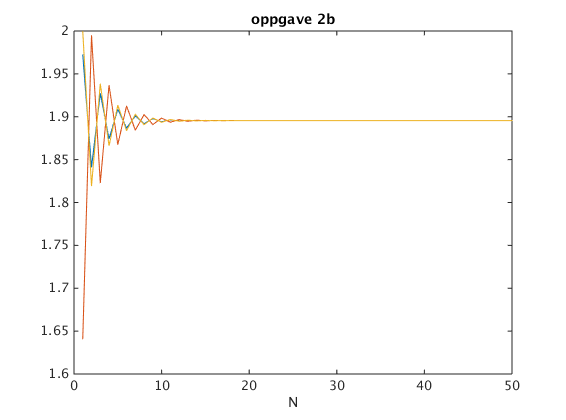
\includegraphics[width=13cm]{oppg2b}
		\end{figure}
	\noindent I starten er ser man en tydelig amplitude på kurven rundt senterlinjen $y = 1.9$, men lar vi følgen løpe litt ser vi fort at amplituden rasktnærmer seg 0.
	\subsection*{}
		\begin{figure}[H]
			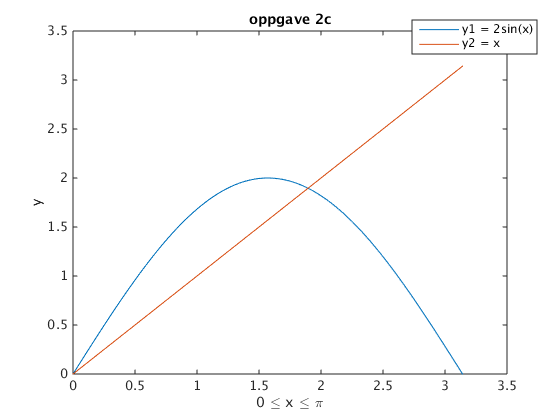
\includegraphics[width=13cm]{oppg2c}
		\end{figure}
		\noindent Leser fra figuren og ser at kurvene skjærer hverandre i punktet. $x\approx1.9$, $y\approx1.9$
	\subsection*{}
		\begin{figure}[H]
			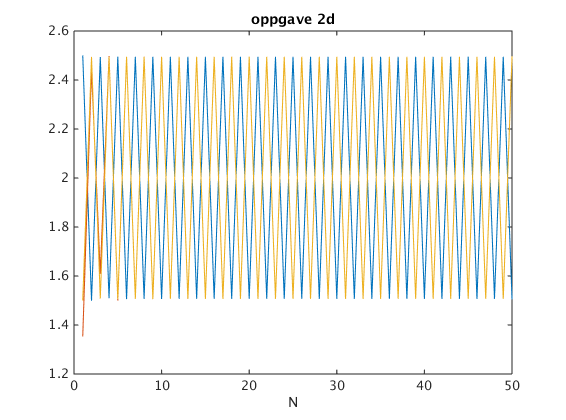
\includegraphics[width=13cm]{oppg2d}
		\end{figure}
		\noindent Stabiliserer seg veldig rask på en peak-to-peak-amplitude $ = 1$, senterlinjen ligger denne gangen på $y = 2$.
	\subsection*{}
		\begin{figure}[H]
			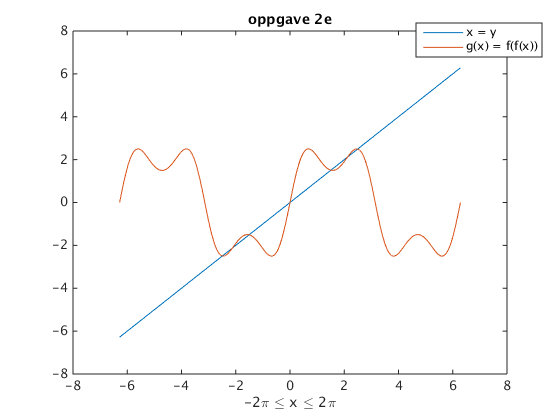
\includegraphics[width=13cm]{oppg2e}
		\end{figure}
		\noindent Leser fra figuren og ser at skjæringspunktene har periodevis verdier, med 1 ved $y\approx0$, 2 ved $\approx2$, 1 ved $y\approx0$ og tilslutt 2 ved $y\approx-2$ før mønsteret gjentar seg. Skjæringspunktene befinner seg på $\pm x\approx0\wedge1\wedge2\wedge3\wedge4\wedge5$
	\subsection*{}
		\begin{figure}[H]
			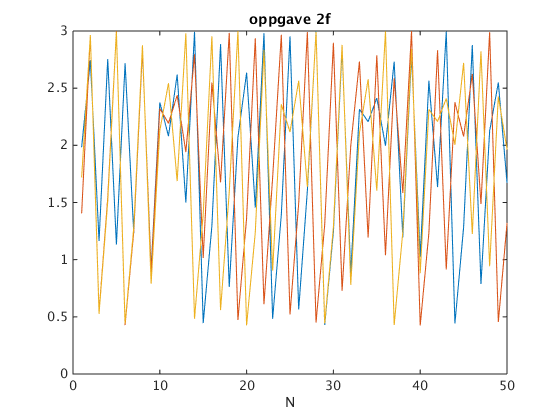
\includegraphics[width=13cm]{oppg2f}
		\end{figure}
		\noindent Ikke godt å si hva som skjer her. Amplituden til den blå grafen roer seg litt periodevis ved $N\approx12$ og $N\approx35$. 
	\subsection*{kode fra oppgave 2}
			\begin{figure}[H]
				\lstinputlisting[language=matlab, frame=single, title=\lstname]{oppg2b.m}
			\end{figure}
			\begin{figure}[H]
				\lstinputlisting[language=matlab, frame=single, title=\lstname]{oppg2c.m}
			\end{figure}
			\begin{figure}[H]
				\lstinputlisting[language=matlab, frame=single, title=\lstname]{oppg2d.m}
			\end{figure}
			\begin{figure}[H]
				\lstinputlisting[language=matlab, frame=single, title=\lstname]{oppg2e.m}
			\end{figure}
			\begin{figure}[H]
				\lstinputlisting[language=matlab, frame=single, title=\lstname]{oppg2f.m}
			\end{figure}
\end{document}